\documentclass[preprint,12pt]{elsarticle}
\biboptions{sort&compress}
\usepackage{amsmath}
\usepackage{amsfonts}
\usepackage{amssymb}
\usepackage{graphicx}
\usepackage{hyperref}
\usepackage{tabls}
\usepackage{multirow}
\usepackage{cleveref}
\usepackage{verbatim}

\usepackage{pgfplots}
\usetikzlibrary{plotmarks}
\usepackage{tikz}
\usetikzlibrary{shapes,arrows}
\newcommand*{\h}{\hspace{5pt}}% for indentation
\newcommand*{\hh}{\h\h}% double indentation

\usepackage{framed} % Framing content
\usepackage{multicol} % Multiple columns environment
\usepackage{nomencl} % Nomenclature package
\RequirePackage{ifthen}
\renewcommand{\nomgroup}[1]{%
\ifthenelse{\equal{#1}{P}}{\item[\textbf{Superscripts}]}{
\ifthenelse{\equal{#1}{G}}{\item[\textbf{Greek Symbols}]}{
\ifthenelse{\equal{#1}{S}}{\item[\textbf{Subscripts}]}{}}}}

\newcommand{\nomunit}[1]{%
\renewcommand{\nomentryend}{\hspace*{\fill}#1}}
\newcommand{\bv}[1]{\boldsymbol #1}  % change this to change how math vectors are handled

%\usepackage{breqn}

%\special{papersize=8.5in,11in}

\journal{International Journal of Heat and Mass Transfer}


\pdfinfo{%
  /Title(Inverse Solution of a Jet in Crossflow by a Predictor-Corrector Technique)
  /Author   (Yogesh Jaluria)
    /Author   (Joseph R VanderVeer)
  /Creator  (Joseph R VanderVeer)
  /Subject  (Inverse Convection Problems)
}

\begin{document}

\begin{frontmatter}
\title{Solution of the Inverse Jet in a Crossflow Problem by a Predictor-Corrector Technique}

\author{Joseph R VanderVeer}
\author{Yogesh Jaluria\corref{cor}}
\ead{jaluria@soemail.rutgers.edu}

\address{Department of Mechanical and Aerospace Engineering: Rutgers University, 98 Brett Rd, Piscataway NJ, 08854}
\cortext[cor]{Corresponding Author}



\begin{abstract}
A predictor-corrector method, developed early, was modified to suit the inverse jet flow in a crosswind problem.  The methodology was tested against both numerical and experimental data.  The jet was generated by heating compressed air with a velocity range of $0-5\,m/s$ and temperatures up to $425\,K$.  The method attempts to predict the jet velocity, temperature, inlet axial location, and elevation with a self imposed limitation on the number of sample points within the domain.  The case where all four of the parameters are unknown led to inaccurate and unacceptable results with 9 sample points.  The thermal self-similarity of the problem results in an infinite number of solutions to the problem, with no possibility of narrowing the solution count without more information.  Knowing the elevation of the jet results in a maximum error of $9\%$, but typically much better.  Experimental tests indicate the methodology is sensitive to error in the sampling data with a few cases reaching an error over $20\%$.  This technique may be extended to applied areas such as exhaust stacks and fuel injection systems.

\end{abstract}
\begin{keyword}
Inverse Problems \sep Computational Heat Transfer \sep Convection
\end{keyword}
\end{frontmatter}

\crefname{equation}{equation}{equations}
\crefname{figure}{figure}{figures}
\crefname{table}{table}{tables}

\newlength\figureheight 
\newlength\figurewidth 
	
	
	
	
\makenomenclature
\setlength{\nomitemsep}{-\parskip} % Baseline skip between items
\renewcommand*\nompreamble{\begin{multicols}{2}}
\renewcommand*\nompostamble{\end{multicols}}
\nomenclature[A]{$T$}{temperature}
\nomenclature[G]{$\bv{\Delta}$}{relative difference between the first sampled point and other sampled points}
\nomenclature[A]{$\bv{r}$}{vector location of sampled points}
\nomenclature[A]{$F$}{minimization function for temperature}
\nomenclature[A]{$G$}{minimization function for velocity}
\nomenclature[A]{$n$}{number of sample locations}
\nomenclature[G]{$\bv{\delta}$}{vector distance between the actual sampled location and the current test location}
\nomenclature[G]{$\varepsilon$}{error associated with the inverse convection method at a location with given sampled data}
\nomenclature[A]{$d$}{number of simulations}
\nomenclature[A]{$a$}{number of sample locations used in the predictor stage}
\nomenclature[A]{$U$}{free stream velocity}
\nomenclature[A]{$x,y$}{coordinates}
\nomenclature[G]{$\phi$}{normalized temperature $\phi = \frac{T-T_{\infty}}{T_S-T_{\infty}}$}
\nomenclature[A]{$X,Y$}{normalized coordinates}
\nomenclature[S]{$i, j,k$}{index}
\nomenclature[S]{$A,B$}{data set A,B}
\nomenclature[S]{$P$}{predicted}
\nomenclature[S]{$mod$}{modified}
\nomenclature[S]{$\infty$}{free stream}
\nomenclature[P]{$\ast$}{predictor stage, alternative heat flux eqn.}
\nomenclature[S]{$S$}{source}
\nomenclature[A]{$b,m,\Gamma_0, \Gamma_1, \Gamma_2$}{model parameters}
\nomenclature[S]{$0,1,2$}{sample point indexes}
\nomenclature[G]{$\rho$}{density}
\nomenclature[A]{$E$}{thermal energy}
\nomenclature[G]{$\mu_{t}$}{eddy viscosity}
\nomenclature[A]{$P_{rt}$}{turbulent Prandtl number}
\nomenclature[A]{$k,\epsilon$}{turbulence kinetic energy, dissipation rate}
\nomenclature[A]{$C_1,C_2,C_{1\epsilon},C_{\mu},\sigma_k,\sigma_{\epsilon}$}{$k-\epsilon$ model coefficients}
\nomenclature[A]{$l, I$}{turbulence length scale and intensity}
\nomenclature[G]{$\lambda$}{thermal conductivity}
\nomenclature[G]{$\mu$}{dynamic viscosity}

%\nomenclature[A]{ }{ }

\begin{table*}[!t]
  \begin{framed}
    \printnomenclature
  \end{framed}
\end{table*}




\section{Introduction}
Thermal-fluid systems often create situations in which the engineering problem is an inverse heat transfer problem.  These problems often have limited physical access, very limited to no boundary condition knowledge, and/or limited domain information.

For example, the temperature distribution at the wall of an optical fiber drawing furnace is difficult to measure directly due to shape, inaccessibility, and high temperatures.  The center of the furnace is easily accessible, where the temperature distribution on an inserted rod may be measured. This leads to the inverse heat transfer problem to obtain the wall temperature distribution that gives rise to the measured rod temperature distribution.  \Citet{issa} developed a regularization technique, utilizing this approach, to determine the wall temperature distribution.

The inverse convection problems have been gaining popularity as of late.  \Citet{inversecgm} solved transient inverse convection problems with a single sensor utilizing the conjugate gradient method, but the sensor needed to be moved closer to the boundary layer as the Rayleigh number increased.  A partially adiabatic enclosure with heat loss was solved.  \Citet{liu} determined the thermal profiles in a slot vented enclosure, also utilizing the conjugate gradient approach, requiring tens of iterations to achieve less than $1\%$ error.  \Citet{inverseconvrad} solved the inverse problem of a differentially heated enclosure with constant wall temperatures.  They demonstrated that using the conjugate gradient method required at least nine sample points to resolve the heat flux into the enclosure.  The conjugate gradient method is a popular method for solving inverse convection problems and is used a number of other works (e.g. \cite{inversecgm,inversesource,inverseenclosure,liu,inverseconvrad}).

A different approach is that of the artificial neural network to solve the inverse heat transfer problem.  Both \citet{conductionneural,inverseneuralnet} successfully applied the technique.  \Citet{conductionneural} solved for the heat conduction in a plate.  While \citet{inverseneuralnet} solved a similar differentially heated enclosure as \cite{inverseconvrad}.  Although requiring more sample points than \cite{inverseconvrad} the technique once trained is non-iterative and thus, typically quicker.

Another example is the inverse plume in a crossflow problem.  The problem entails solving for the plume boundary conditions, utilizing limited domain knowledge.  A novel predictor-corrector method was developed by \citet{ijhmt1} to solve such a problem.  The method requires a specific pattern of known points to match exactly against a set of simulations to predict the inverse solution.  The specific pattern was optimized to require the least number of data points for plume in a crossflow problem \cite{ijhmt2}.  With zero error in the data, a minimum of three known points was possible.  However, small amounts of error, as is usually the case, would require the known point count to increase to at least five.

The present work is the logical progression of the inverse plume in a crossflow problem, that is the inverse jet in a crossflow problem.  The inverse jet in a crossflow problem has many more practical applications, such as exhaust stacks and fuel injection systems.  The previous technique will be modified to meet the needs of the new problem.


\section{Experimental System}
The experiment consists of a wind tunnel with a surface level jet located within the test section.  The jet uses compressed air flowing through straighteners to achieve a velocity $U_S$ and is heated to temperature $T_S$.  The jet is subjected to a perpendicular crossflow velocity $U_{\infty}$.  \Cref{fig:diagramjet} is a diagram of the wind tunnel and the jet, with dimensions in millimeters.

\begin{figure}[!tbp]
\begin{center}
\includegraphics[scale=.30]{windtunneljet.jpg}
\caption{Schematic of a jet in a wind tunnel}
\label{fig:diagramjet}
\end{center}
\end{figure}

The wind tunnel test section dimensions are $54.5\times305\times 254\,mm$.  The maximum velocity of the wind tunnel is $5.0\,m/s$.  The jet is heated by electric cartridge heaters (Omega AHP-7561) with a maximum temperature of $425\,K$, due to material limitations of the wind tunnel.  The X-direction is directed downstream of the wind tunnel with the zero at the center of the jet.  The Y-direction is in the direction of the jet and is zero at the surface of the wind tunnel.  Due to the large aspect ratio of the wind tunnel $\approx\left(5:1\right)$, the flow is assumed to be two-dimensional.

The free stream velocity is determined by a Pitot-Static tube attached to a NIST traceable differential pressure sensor from Omega(PX655-0.1DI).  The pressure sensor has a full scale reading of $2.54\,mm$ of water and is accurate to $0.05\%$ of full scale.  This results in a maximum error of $3\%$ in the calculated velocity.  The jet velocity is determined utilizing a rotameter and verified using a Pitot-Static tube attached to the same previously described pressure sensor.  This results in the same amount of error in the jet velocity.

The temperature of domain is measured using a K-type thermocouple mounted to an X-Y traversing stage.  Sampled data over the course of several days indicate repeatability of the experiment to within $2\%$.

\section{Numerical Simulations}
The simulations were all performed using Ansys Fluent\cite{fluentsoftware}.  The Navier-Stokes equations were solved using a three-dimensional, steady state, realizable $k-\epsilon$ model with enhanced wall effects.  Conjugate heat transfer effects are modeled.  The free stream Reynolds number $Re_{infty}$ is of order $6\times10^3$, while the jet Reynolds number $Re_S$ is between $10^3$ and $10^4$.  The Rayleigh number $Ra$ is of order $10^7$.

The governing equations are expressed below:

\begin{equation}
\centering
u_i = \overline{u_i} + u^{'}_{i}
\label{eq:veldecomp}
\end{equation}

\begin{equation}
\frac{\partial \rho }{\partial t } + \frac{\partial }{\partial x_i} \left( \rho u_i \right) = 0 
\label{eq:mass}
\end{equation}

\begin{equation}
\centering
\begin{split}
\frac{\partial }{\partial t} \left( \rho u_i \right) &+ \frac{\partial }{\partial x_j } \left( \rho u_i u_j \right) = \\
 &\frac{\partial P}{\partial x_i } + \frac{\partial }{\partial x_j } \left[ \mu \left( 2 S_{ij} - \frac{2}{3} \delta_{ij} \frac{\partial u_k }{\partial x_k } \right) - \rho \overline{u^{'}_{i} u^{'}_{j}} \right] 
\label{eq:momentum}
\end{split}
\end{equation}

\begin{equation}
\centering
\begin{split}
\frac{\partial }{\partial t } \left( \rho E \right) &+ \frac{\partial }{\partial x_i} \left[ u_i \left( \rho E + P \right) \right] = \\
 &\frac{\partial }{\partial x_i } \left[ \left( \lambda + \frac{C_p \mu_t }{P_{rt}} \right) \frac{\partial T}{\partial x_i} \right] 
\label{eq:energy}
\end{split}
\end{equation}

\begin{equation}
\centering
\begin{split}
\frac{\partial }{\partial t} \left(\rho k \right) &+ \frac{\partial }{\partial x_j} \left( \rho k u_j \right) = \\
&\frac{\partial }{\partial x_j} \left[ \left( \mu + \frac{\mu_t}{\sigma_k} \right) \frac{\partial k}{\partial x_j} \right] + \frac{\partial u_j}{\partial x_i} \left( -\rho \overline{u^{'}_{i} u^{'}_{j}} \right) \\
&- g_i \frac{\mu_t}{\rho P_{rt}} \frac{\partial \rho }{\partial x_i} + \rho \epsilon
\label{eq:k}
\end{split}
\end{equation}

\begin{equation}
\centering
\begin{split}
 \frac{\partial }{\partial t} \left(\rho \epsilon \right) &+ \frac{\partial }{\partial x_j} \left( \rho \epsilon u_j \right) = \\
 &\frac{\partial }{\partial x_j } \left[ \left( \mu + \frac{\mu_t }{\sigma_\epsilon } \right) \frac{\partial \epsilon }{\partial x_j } \right] + \rho C_1 S \epsilon - \rho C_2 \frac{\epsilon^2 }{k+\sqrt{\nu \epsilon}} \\
 &- C_{1 \epsilon} \frac{\epsilon}{k} C_{3\epsilon} g_i \frac{\mu_t}{\rho P_{rt}} \frac{\partial \rho}{\partial x_i}
\label{eq:e}
\end{split}
\end{equation}

\begin{equation}
\centering
- \rho \overline{u^{'}_{i} u^{'}_{j}} = 2\mu_t S_{ij} - \frac{2}{3} \delta_{ij} \left( \rho k + \mu_t \frac{\partial u_k}{\partial x_k} \right)
\label{eq:reynoldsstress}
\end{equation}

The constants for the turbulence model are \cite{realizable,fluent} : 
\begin{equation}
\label{eq:constants}
C_{1\epsilon} = 1.44 , C_2 = 1.9 , \sigma_k = 1.0 , \sigma_\epsilon = 1.2 , P_{rt} = 0.85 
\end{equation}
\begin{equation}
C_1 = max\left[0.43,\frac{Sk/\epsilon}{Sk/\epsilon +5} \right] , S = \sqrt{2S_{ij}S_{ji}} , C_{3\epsilon} = tanh\left(\frac{u_g}{u_p}\right)
\end{equation}
\begin{subequations}
\begin{align}
\mu_t &= \frac{\rho C_{\mu} k^2}{\epsilon} \\
C_{\mu} &= \frac{1}{A_0 + \frac{A_1 k U^*}{\epsilon}} \\
U^* &\equiv \sqrt{S_{ij} S_{ji} + \Omega_{ij} \Omega_{ji}} \\
A_0 &= 4.04 \\
A_1 &= \sqrt{6} cos \left[\frac{1}{3} cos^{-1}\left(\sqrt{6} \frac{S_{ij}S_{jk}S_{ki}}{\left(S_{ij} S_{ji} \right)^{\frac{3}{2}}} \right) \right] \\
S_{ij} &= \frac{1}{2} \left( \frac{\partial u_i}{\partial x_j} + \frac{\partial u_j}{\partial x_i} \right) \\
\Omega_{ij} &= \frac{1}{2} \left( \frac{\partial u_i}{\partial x_j} - \frac{\partial u_j}{\partial x_i} \right)
\end{align}
\end{subequations}
where the $u_g$ and $u_p$ are the velocity component parallel and perpendicular to gravity respectively.  All of the symbols are defined in the nomenclature.

The inflow boundary conditions are:
\begin{subequations}
\label{eq:inflow}
\begin{align}
u&=U_\infty , v=0 , T=T_\infty , P = P_\infty , l=4 mm , I=5\%\\
k&=\frac{3}{2}\left(U_\infty I\right)^2 \\
\epsilon &=C_{\mu}^{3/4} \frac{k^{3/2}}{l}
\end{align}
\end{subequations}

The jet inflow boundary conditions are:
\begin{subequations}
\label{eq:inflowjet}
\begin{align}
u&=0 , v=U_S , T=T_S , P = P_\infty , l=4 mm , I=5\%\\
k&=\frac{3}{2}\left(U_\infty I\right)^2 \\
\epsilon &=C_{\mu}^{3/4} \frac{k^{3/2}}{l}
\end{align}
\end{subequations}

The upper boundary is very far from the jet and therefore should have negligible effect on the numerical result.  Thus, the boundary was taken to be symmetric to reduce the possibility of errors by the experimentally accurate no-slip condition.  The outflow boundary is at the pressure $P_{\infty}$.  The wind tunnel walls are $12\, mm$ thick acrylic, while the test section bottom is modeled as $25.4\,mm$ thick acrylic.  The external boundary conditions are isothermal with a temperature of $T_{\infty}$.  The test section bottom external temperature is modeled as isothermal $\frac{1}{2}\left(T_S+T_{\infty}\right)$.  This temperature is used to attempt to model the complicated geometry of the test section floor.  Two sheets of acrylic are separated by a small air gap of approximately $0.75\,mm$ and the exterior sheet is exposed to jet temperature air.  While not ideal, the experimental-numerical comparisons, shown later, demonstrate this is a reasonable model.

\subsection{Simulation Validation}
A simulation validation study was performed to verify the results of the simulations.  Typical verification was performed including flow model, grid independence, and comparison with experimental results.  The conditions of the simulation validation are shown in \cref{tab:VTjet}.

\begin{table}[!t!b!p]
\begin{center}
\begin{tabular}{ c c }
\hline
Parameter    & Value \\ \hline
$U_{\infty} \, (m/s)$ & $2.0\pm0.02$ \\
$U_S \, (m/s)$ & $2.0\pm0.2$ \\
$T_{\infty} \, (K) $ & $305\pm0.5$ \\
$P_{\infty} \, (kPa) $ & $101.3\pm0.01$ \\
$T_{S} \, (K) $ & $350\pm2.0$ \\ \hline
\end{tabular}
\caption{Validation test conditions}
\label{tab:VTjet}
\end{center}
\end{table}

The results from Spalart-Allmaras(SA), $k-\epsilon$, and $k-\omega$ were compared and the three models have similar trends.  SA tends to be a bit off, but this is expected due to issues SA has with shear flows, especially plane jets\cite{fluent}.  All of the values were normalized utilizing \cref{eq:normal}, where $D$ is the width of the jet.  \Cref{fig:jetmodel15mm} shows a comparison of the results from the flow models at $X=4.75$.
\begin{subequations}
\begin{align}
\phi &= \frac{T-T_{\infty}}{T_S-T_{\infty}} \\
X &= \frac{x}{D} \\
Y &= \frac{y}{D} \\
V &= \frac{U}{U_\infty}  \\
V_S &= \frac{U_S}{U_{\infty}}
\end{align}
\label{eq:normal}
\end{subequations}
\begin{figure}[!tbp]
	\centering
  \setlength\figureheight{5cm} 
	\setlength\figurewidth{5cm}
	% This file was created by matlab2tikz v0.2.1.
% Copyright (c) 2008--2012, Nico Schlömer <nico.schloemer@gmail.com>
% All rights reserved.
% 
% The latest updates can be retrieved from
%   http://www.mathworks.com/matlabcentral/fileexchange/22022-matlab2tikz
% where you can also make suggestions and rate matlab2tikz.
% 
% 
% 
\begin{tikzpicture}

\begin{axis}[%
view={0}{90},
width=\figurewidth,
height=\figureheight,
scale only axis,
xmin=0, xmax=0.8,
xlabel={Normalized Temperature},
ymin=0, ymax=5,
ylabel={Normalized Distance Above Surface (Y-axis)},
axis lines=left,
legend style={nodes=right}]
\addplot [
color=black,
dashed,
line width = 1.5pt
]
coordinates{
 (0.598022194358906,0)(0.719633644440864,0.31496062992126)(0.773342793297479,0.62992125984252)(0.787137560078285,0.94488188976378)(0.786982506712231,1.25984251968504)(0.767485577679692,1.5748031496063)(0.716462238981407,1.88976377952756)(0.621973697060202,2.20472440944882)(0.480706343310905,2.51968503937008)(0.311097850416844,2.83464566929134)(0.160803897231797,3.1496062992126)(0.0691451576006809,3.46456692913386)(0.0249505232734139,3.77952755905512)(0.00763753550304175,4.09448818897638)(0.00197928210192474,4.40944881889764)(0.000359340398558418,4.7244094488189) 
};

\addlegendentry{SA};

\addplot [
color=black,
solid,
line width = 1.5pt
]
coordinates{
 (0.475508101325801,0)(0.550052890287577,0.31496062992126)(0.55412002610574,0.62992125984252)(0.531443362113594,0.94488188976378)(0.496125463740959,1.25984251968504)(0.450496289862748,1.5748031496063)(0.3934550283275,1.88976377952756)(0.328670791774968,2.20472440944882)(0.262813124212552,2.51968503937008)(0.199826985242342,2.83464566929134)(0.143142443504267,3.1496062992126)(0.0963463996907779,3.46456692913386)(0.0601829585553529,3.77952755905512)(0.0358385592290458,4.09448818897638)(0.0192371842163784,4.40944881889764)(0.00922113373690982,4.7244094488189) 
};

\addlegendentry{k-e};

\addplot [
color=black,
dotted,
line width = 1.5pt
]
coordinates{
 (0.623553431329684,0)(0.72099881236359,0.31496062992126)(0.751725742420293,0.62992125984252)(0.769701953149541,0.94488188976378)(0.779485121151673,1.25984251968504)(0.770323219262517,1.5748031496063)(0.724627008448031,1.88976377952756)(0.628332228898429,2.20472440944882)(0.472876701362613,2.51968503937008)(0.283070581920853,2.83464566929134)(0.133380285447469,3.1496062992126)(0.0586545740916514,3.46456692913386)(0.0258944594893283,3.77952755905512)(0.012059155531458,4.09448818897638)(0.0058223208773638,4.40944881889764)(0.00276500998016413,4.7244094488189) 
};

\addlegendentry{k-w};

\end{axis}
\end{tikzpicture}

	\caption{Validation of the simulation: local temperature using three flow models at $X=4.75$}
	\label{fig:jetmodel15mm}
\end{figure}

Grid independence is demonstrated by testing the temperature at a few locations with various grid sizes and geometries, as shown in \cref{tab:gridjet}.  Very little variation in simulated temperature over such a wide variety of cell counts shows that the result is essentially grid independent.  The grid employed is an unstructured hexagonal mesh with refinement located near the jet and down stream of the jet.
\begin{table}[!t!b!p]
\begin{center}
\begin{tabular}{ c c c c c }
\hline
 Location (x,y) (mm) & 0,1 & 10,5 & 15,5& 30,10 \\ \hline \hline
 Cell Count & \\ \hline
 57660  & 337.7 & 323.3 & 321.6 & 310.1 \\ \hline
 83888  & 337.7 & 323.3 & 321.6 & 310.1 \\ \hline
 166352 & 337.7 & 323.2 & 321.5 & 310.1 \\ \hline
 366168 & 337.7 & 323.2 & 321.5 & 310.1 \\ \hline
\end{tabular}
\caption{Grid Independence Study, local static temperature (K)}
\label{tab:gridjet}
\end{center}
\end{table}

%Iterative convergence is typically proven by increasing the residual requirements to very tiny amounts.  In this case, due to the extremely small elements within the jet, a residual of $10^{-8}$ was used.  \Cref{fig:jetiterate15mm} is a plot of error compared to the $10^{-8}$ residuals for several residual cases.  It can be seen that the error is progressively reducing and a residual of $10^{-6}$ should give acceptable iterative errors (experimental - numerical errors will be much larger).
%\begin{figure}[!htbp]
%	\centering
%  \setlength\figureheight{5cm} 
%	\setlength\figurewidth{5cm}
%	% This file was created by matlab2tikz v0.2.1.
% Copyright (c) 2008--2012, Nico Schlömer <nico.schloemer@gmail.com>
% All rights reserved.
% 
% The latest updates can be retrieved from
%   http://www.mathworks.com/matlabcentral/fileexchange/22022-matlab2tikz
% where you can also make suggestions and rate matlab2tikz.
% 
% 
% 
\begin{tikzpicture}

\begin{semilogyaxis}[%
view={0}{90},
width=\figurewidth,
height=\figureheight,
scale only axis,
xmin=0, xmax=5,
xlabel={Normalized distance above surface (Y-axis)},
ymin=1e-07, ymax=1,
yminorticks=true,
ylabel={$\text{Error in temperature from 10}^\text{-8}\text{ residual solution}$},
legend style={at={(0.97,0.03)},anchor=south east,nodes=right}]
\addplot [
color=black,
solid,
line width = 1.5pt
]
coordinates{
 (0,0.183570039895699)(0.31496062992126,0.119677394602206)(0.62992125984252,0.0597678374185762)(0.94488188976378,0.0418913694597904)(1.25984251968504,0.0546738639469027)(1.5748031496063,0.111687747425776)(1.88976377952756,0.214670181029362)(2.20472440944882,0.305412872110992)(2.51968503937008,0.366805042231704)(2.83464566929134,0.415767406934549)(3.1496062992126,0.462479217653083)(3.46456692913386,0.482454684632103)(3.77952755905512,0.43377134001264)(4.09448818897638,0.33854894473302)(4.40944881889764,0.245785109674443)(4.7244094488189,0.194837795539684) 
};

\addlegendentry{$\text{10}^\text{-3}\text{ residual solution}$};

\addplot [
color=black,
dashed,
line width = 1.5pt
]
coordinates{
 (0,0.0151811582664436)(0.31496062992126,0.00883978518027106)(0.62992125984252,0.0633427719325255)(0.94488188976378,0.115325317676366)(1.25984251968504,0.168642968325742)(1.5748031496063,0.224728800892933)(1.88976377952756,0.282436260197301)(2.20472440944882,0.326207842677263)(2.51968503937008,0.346915060896265)(2.83464566929134,0.341730467759419)(3.1496062992126,0.304920656577735)(3.46456692913386,0.238907388975122)(3.77952755905512,0.158557517611655)(4.09448818897638,0.0877039804846618)(4.40944881889764,0.0323108499647446)(4.7244094488189,0.000135787316366986) 
};

\addlegendentry{$\text{10}^\text{-4}\text{ residual solution}$};

\addplot [
color=black,
dotted,
line width = 1.5pt
]
coordinates{
 (0,0.00301340971111586)(0.31496062992126,0.000847562800913693)(0.62992125984252,0.00989423149235336)(0.94488188976378,0.018617114346398)(1.25984251968504,0.0276829545532564)(1.5748031496063,0.037338349823699)(1.88976377952756,0.0474188540300702)(2.20472440944882,0.0550364719680374)(2.51968503937008,0.0587359020376539)(2.83464566929134,0.0581153888354606)(3.1496062992126,0.0523245346329873)(3.46456692913386,0.0416577979382282)(3.77952755905512,0.0284490337069201)(4.09448818897638,0.0165378768803066)(4.40944881889764,0.00693834451902831)(4.7244094488189,0.00113070810812133) 
};

\addlegendentry{$\text{10}^\text{-5}\text{ residual solution}$};

\addplot [
color=black,
dash pattern=on 1pt off 3pt on 3pt off 3pt,
line width = 1.5pt
]
coordinates{
 (0,0.000688085826709539)(0.31496062992126,0.00010438255480949)(0.62992125984252,0.00202450657644704)(0.94488188976378,0.00398273992459508)(1.25984251968504,0.0060003200499068)(1.5748031496063,0.00832188350352681)(1.88976377952756,0.0108006902906936)(2.20472440944882,0.0127447780458283)(2.51968503937008,0.0137839565915101)(2.83464566929134,0.0138214406717907)(3.1496062992126,0.0127810643082853)(3.46456692913386,0.0106045271317043)(3.77952755905512,0.00779861894483247)(4.09448818897638,0.00511043713959225)(4.40944881889764,0.00278143168583256)(4.7244094488189,0.00124559922232947) 
};

\addlegendentry{$\text{10}^\text{-6}\text{ residual solution}$};

\addplot [
color=black,
dash pattern=on 1pt off 3pt on 3pt off 3pt,
mark=*,
mark options={solid},
line width = 1.5pt
]
coordinates{
 (0,7.77858267611009e-05)(0.31496062992126,4.61006607110903e-07)(0.62992125984252,0.00023318715568621)(0.94488188976378,0.000524454380752104)(1.25984251968504,0.000763280193268656)(1.5748031496063,0.00109295503034446)(1.88976377952756,0.00140128832242681)(2.20472440944882,0.00166654300102209)(2.51968503937008,0.00182302902118181)(2.83464566929134,0.00181343901658693)(3.1496062992126,0.00167711899092637)(3.46456692913386,0.00140236689549056)(3.77952755905512,0.00105344272299135)(4.09448818897638,0.000725345661692245)(4.40944881889764,0.000423700675810323)(4.7244094488189,0.000215679471637031) 
};

\addlegendentry{$\text{10}^\text{-7}\text{ residual solution}$};

\end{semilogyaxis}
\end{tikzpicture}

%	\caption{Validation of the simulation: local temperature error vs residuals set to $10^{-8}$ at $X=4.75$}
%	\label{fig:jetiterate15mm}
%\end{figure}

The final validation is based on comparing the simulation against the experiment carried out in this study.  This is done in \cref{fig:jetexp15}.  The simulation matches the experiment closely, with the exception of very close to the wall.  This is to be expected as the flow models used, even with enhanced wall effects, have difficulty perfectly modeling the near wall conditions.
\begin{figure}[!htbp]
	\centering
	\setlength\figureheight{5cm} 
	\setlength\figurewidth{5cm}
	% This file was created by matlab2tikz v0.2.1.
% Copyright (c) 2008--2012, Nico Schlömer <nico.schloemer@gmail.com>
% All rights reserved.
% 
% The latest updates can be retrieved from
%   http://www.mathworks.com/matlabcentral/fileexchange/22022-matlab2tikz
% where you can also make suggestions and rate matlab2tikz.
% 
% 
% 
\begin{tikzpicture}

\begin{axis}[%
view={0}{90},
width=\figurewidth,
height=\figureheight,
scale only axis,
xmin=0, xmax=0.7,
xlabel={Normalized Temperature},
ymin=0, ymax=9,
ylabel={Normalized Distance Above Surface (Y-axis)},
axis lines=left,
legend style={nodes=right},
unbounded coords=jump]
\addplot [
color=black,
only marks,
mark=o,
mark options={solid}
]
coordinates{
 (0.567284867139084,0)(0.549954067724983,0.535433070866142)(0.472923406467594,1.07086614173228)(0.469207039692354,1.60629921259843)(0.335011020113598,2.14173228346457)(0.193408989244926,2.67716535433071)(0.124031426702604,3.21259842519685)(0.0535628737296839,3.74803149606299)(0.0345607039493489,4.28346456692913)(0.012536305152985,4.81889763779528)(0.00447868470703723,5.35433070866142)(0.00494685782976145,5.88976377952756) 
};

\addlegendentry{Experiment};

\addplot [
color=black,
solid
]
coordinates{
 (0.475508101325801,0)(0.550052890287577,0.31496062992126)(0.55412002610574,0.62992125984252)(0.531443362113594,0.94488188976378)(0.496125463740959,1.25984251968504)(0.450496289862748,1.5748031496063)(0.3934550283275,1.88976377952756)(0.328670791774968,2.20472440944882)(0.262813124212552,2.51968503937008)(0.199826985242342,2.83464566929134)(0.143142443504267,3.1496062992126)(0.0963463996907779,3.46456692913386)(0.0601829585553529,3.77952755905512)(0.0358385592290458,4.09448818897638)(0.0192371842163784,4.40944881889764)(0.00922113373690982,4.7244094488189) 
};

\addlegendentry{Simulation};

\end{axis}
\end{tikzpicture}

	\caption{Validation of the simulation: local temperature - experiment versus simulation at $X=4.75$}
	\label{fig:jetexp15}
\end{figure}

\section{Inverse Solution Methodology}
The basis for the solution strategy was described in the paper by \citet{ijhmt1}, which was intended to solve the inverse plume in a crosswind.  This methodology solved for the 2-D location and source strength of a plume in a crossflow.  The jet in a crossflow solver must handle one additional parameter, the jet velocity.  Therefore the methodology is required to be modified.  For the sake of completeness, the original methodology will be briefly described here.

The method assumed that we can neglect the variations in density, variations in thermal buoyancy, and thermal radiation.  If this is true, then the temperature of a given location ($T\left( \bv r \right)$) is linearly dependent upon the source temperature ($T_S$) as shown in \cref{eq:linearset}.  The two parameters $m$ and $b$ are both location ($\bv{r}$) dependent and may be calculated knowing a unique set of simulations $A$ and $B$.
\begin{subequations}
\label{eq:linearset}
\begin{align}
T_S &= m\left(  \bv r  \right) T\left( \bv r \right) + b\left( \bv r \right) \label{eq:linear} \\
\bv r &= r\left( x, y\right) \label{eq:vector}\\
\bv{r_i} & = \bv{r_0} + \bv{\Delta_i} \label{eq:delta}\\
m\left( \bv r \right) &= \frac{T_{SA} - T_{SB}}{T_A\left( \bv r \right) - T_B\left( \bv r \right)} \label{eq:m} \\
b\left( \bv r \right) &= T_{SA} - m\left( \bv r \right) T_A \left( \bv r \right) \label{eq:b}
\end{align}
\end{subequations}

There are a few quick terms to make the following explanation easier.  Sample point: local static temperature from within the domain at a particular location.  Datum point: a selected sample point whose location will be defined as $\Delta_{0} = (0\,mm,0\,mm)$.  Search shape: relative location and pattern between a set of sample points and a datum point.

Start by selecting $n$ sample points and $d$ simulations.  The method attempts to minimize the discrepancies between all of the sample points' calculated source temperature and the datum point's calculated source temperature to get a predicted source temperature.  Then minimize the discrepancy between the predicted source temperature and a new set of sample point calculated source temperatures to get the corrected location and temperature.  The following equations mathematically describe the previous text.  \Cref{eq:F} is a minimized at $\bv{r^{\ast}_{SP}}$ and the location $\bv{r^{\ast}_{SP}}$ is used to calculate the predicted source temperature in \cref{eq:Tsp}.  Then \cref{eq:Fmod} is minimized at $\bv{r_{SP}}$ and the location $\bv{r_{SP}}$ is calculated with \cref{eq:T} used to calculate $T_{SP}$, where $a$ is the number of sample points used in the prediction step and $n$ is the total number of sample points.
\begin{equation}
\centering
F\left( \bv r \right) =  \sum^{a}_{i=1} [ m\left( \bv r + \bv{\Delta_i}  \right) T\left( \bv{r_i} \right) +b\left( \bv r + \bv{\Delta_i} \right) -m\left( \bv r \right) T\left( \bv{r_0} \right) - b\left( \bv r \right) ]^2  
\label{eq:F}
\end{equation}
%
\begin{equation}
\centering
T^{\ast}_{SP} = \frac{1}{a} \{ \sum^{a}_{i=0} [ m\left( \bv{r^{\ast}_{SP}}+ \bv{\Delta_i}  \right) T\left( \bv{r_i} \right)  + b\left( \bv{r^{\ast}_{SP}}+ \bv{\Delta_i} \right) ] \}
\label{eq:Tsp}
\end{equation}
%
\begin{equation}
\centering
F_{mod}\left( \bv r \right) = \sum^{n}_{i=a} [ m\left( \bv r +\bv{\Delta_i} \right) T\left( \bv{r_i} \right) + b\left( \bv r + \bv{\Delta_i} \right)-T^{\ast}_{SP} ]^2
\label{eq:Fmod}
\end{equation}
%
\begin{equation}
\centering
T_{SP} = \frac{1}{n-a} \{ \sum^{n-a}_{i=a} [ m\left( \bv{r_{SP}}+ \bv{\Delta_i} \right) T\left( \bv{r_i}\right)  + b\left( \bv{r_{SP}}+ \bv{\Delta_i}  \right) ] \}
\label{eq:T}
\end{equation}

The number and pattern of the sample points (i.e. the search shape) was optimized in a paper by \citet{ijhmt2}.  In it three sample points were identified as being enough to solve the inverse plume problem.  The three points were later shown to not handle error very well and the optimization process was continued to include nine sample points.  They are shown in \cref{tab:expoptresults}.
\begin{table}[!h!t!b!p]
\begin{center}
\begin{tabular}{ c c }
\hline
 Sample Point & $\bv{\Delta} \, (mm)$  \\ \hline 
0 & (0.0, 0.0) \\
1 & (1.7, 3.5) \\
2 & (2.8, 0.6) \\  
3 & (0.5, 1.1) \\
4 & (2.1, 1.0) \\ 
5 & (2.3, 2.0) \\
6 & (1.2, 0.8) \\
7 & (3.1, 0.7) \\
8 & (0.8, 2.1) \\ \hline
 \end{tabular}
\caption{Search shape results of averaging over the domain with increasing the sample size to 9}
\label{tab:expoptresults}
\end{center}
\end{table}

Going back to the inverse jet in a crossflow problem, \citet{knight} used a quadratic response surface model to determine the jet temperature and jet velocity.  Unfortunately, the response surface model used is two dimensional and would have difficulty applying directly to the current model.  The response surface models effectiveness does demonstrate the quadratic nature of the jet velocity and linear nature of jet temperature with respect to local temperature.

The method starts similar to the original method, by selecting $n$ sample points and $d$ simulations spanning the thermal and velocity region of interest.  Guess a jet velocity ($U_S$) so the linear parameters are not dependent upon the jet velocity during the minimization.  Calculate the parameters $m$ and $b$ from \cref{eq:linearset}.  Find the minimization of \cref{eq:F} in which we can find a predicted temperature from \cref{eq:Tsp}.  We can develop an equation similar to \cref{eq:F} for the jet velocity.  Starting with \cref{eq:Us}, we can minimize the discrepancy between the predicted jet velocities resulting in \cref{eq:G}.  As would be expected there are three parameters needed ($\Gamma_0,\Gamma_1,\Gamma_2$).  The minimization of $G$ allows $U_{SP}$ to be calculated from \cref{eq:Usp}.  This new $U_{SP}$ is then used to calculated a new set of linear parameters $m$ and $b$.  The process repeats itself until both the change in $U_{SP}$ and the change in $T_{SP}$ is smaller than some small residual.  That is to say $U_{SP}<\epsilon_U$ and $T_{SP}<\epsilon_T$, where $\epsilon_U$ and $\epsilon_T$ are small values such as $0.01\,m/s$ and $0.1\,K$ respectively.  A flowchart of the methodology is shown in \cref{fig:flowchartjet}.



\begin{equation}
\centering
U_S = \Gamma_2 \left(\bv r \right) T\left( \bv r \right)^2 +  \Gamma_1 \left(\bv r \right) T\left( \bv r \right) + \Gamma_0 \left(\bv r \right)
\label{eq:Us}
\end{equation}
%
\begin{equation}
\centering
\begin{split}
G\left( \bv r \right) =  \sum^{n}_{i=a} [ &\Gamma_2\left( \bv r + \bv{\Delta_i}  \right) T\left( \bv{r_i} \right)^2 \\
&+\Gamma_1\left( \bv r + \bv{\Delta_i}  \right) T\left( \bv{r_i} \right) \\
&+\Gamma_0\left( \bv r + \bv{\Delta_i} \right) \\
&-\Gamma_2\left( \bv r \right) T\left( \bv{r_0} \right)^2 \\
&-\Gamma_1\left( \bv r \right) T\left( \bv{r_0} \right)\\
&- \Gamma_0\left( \bv r \right) ]^2  
\label{eq:G}
\end{split}
\end{equation}
%
\begin{equation}
\centering
\begin{split}
U_{SP} = \frac{1}{n-a} \{ \sum^{n-a}_{i=a} [ &\Gamma_2 \left( \bv{r_{SP}}+ \bv{\Delta_i} \right) T\left( \bv{r_i}\right)^2  \\
&+\Gamma_1 \left( \bv{r_{SP}}+ \bv{\Delta_i} \right) T\left( \bv{r_i}\right) \\
&+ \Gamma_0\left( \bv{r_{SP}}+ \bv{\Delta_i}  \right) ] \}
\label{eq:Usp}
\end{split}
\end{equation}

\begin{figure}[!tbp]
\centering
  % setting the typeface to sans serif and the font size to small
  % the scope local to the environment
  \sffamily
  \footnotesize
  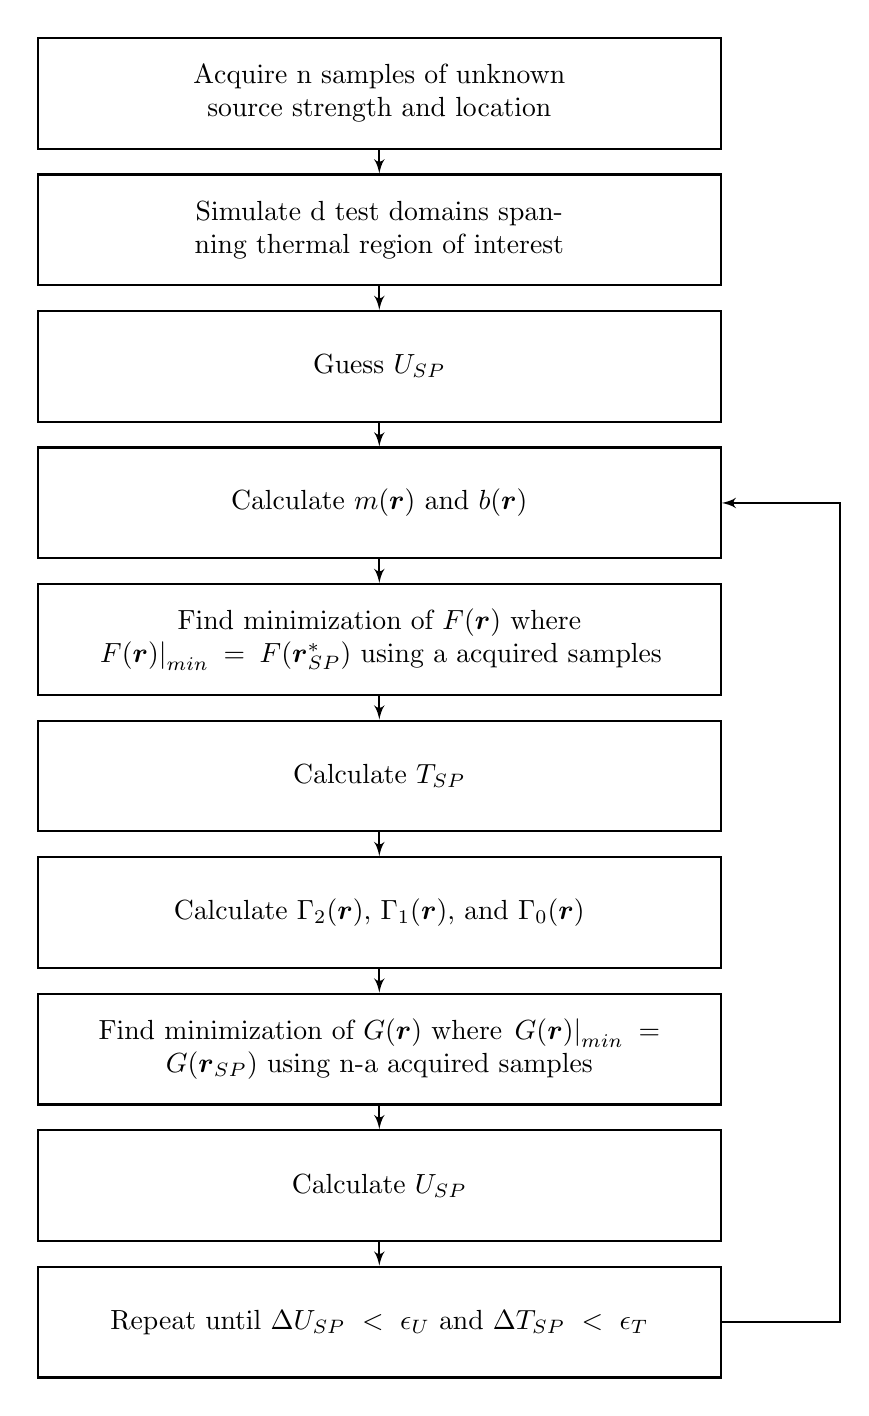
\begin{tikzpicture}[auto,
    %decision/.style={diamond, draw=black, thick, fill=white,
    %text width=8em, text badly centered,
    %inner sep=1pt, font=\sffamily\small},
    block_center/.style ={rectangle, draw=black, thick, fill=white,
      text width=24em, text centered,
      minimum height=4em},
    block_left/.style ={rectangle, draw=black, thick, fill=white,
      text width=16em, text ragged, minimum height=4em, inner sep=6pt},
    block_noborder/.style ={rectangle, draw=none, thick, fill=none,
      text width=18em, text centered, minimum height=1em},
    block_assign/.style ={rectangle, draw=black, thick, fill=white,
      text width=18em, text ragged, minimum height=3em, inner sep=6pt},
    block_lost/.style ={rectangle, draw=black, thick, fill=white,
      text width=16em, text ragged, minimum height=3em, inner sep=6pt},
      line/.style ={draw, thick, -latex', shorten >=0pt}]
    % outlining the flowchart using the PGF/TikZ matrix funtion
    \matrix [column sep=5mm,row sep=3mm] {
			\node [block_center] (acquire) {Acquire n samples of unknown source strength and location};\\
		  \node [block_center] (sim) {Simulate d test domains spanning thermal region of interest};	\\		
		  \node [block_center] (jet) {Guess $U_{SP}$};	\\				  
			\node [block_center] (calcm) {Calculate $m( \bv r)$ and $b( \bv r)$};	\\		
			\node [block_center] (minf) {Find minimization of $F( \bv r)$ where $\left. F( \bv r) \right|_{min} = F(\bv{r^{\ast}_{SP}})$ using a acquired samples};	\\					
			\node [block_center] (calcts) {Calculate $T_{SP}$};	\\		
			\node [block_center] (calca) {Calculate $\Gamma_2( \bv r)$, $\Gamma_1( \bv r)$, and $\Gamma_0( \bv r)$};	\\		
			\node [block_center] (ming) {Find minimization of $G(\bv r)$ where $\left. G( \bv r) \right|_{min} = G(\bv{r_{SP}})$ using n-a acquired samples};	\\					
			\node [block_center] (calcu) {Calculate $U_{SP}$};	\\					
			\node [block_center] (repeat) {Repeat until $\Delta U_{SP} < \epsilon_U$ and $\Delta T_{SP} < \epsilon_T$};	\\					
   };% end matrix
    % connecting nodes with paths
    \begin{scope}[every path/.style=line]
      \path (acquire)     -- (sim);
			\path (sim)     -- (jet);
			\path (jet)     -- (calcm);			
			\path (calcm)     -- (minf);
			\path (minf)     -- (calcts);			
			\path (calcts)     -- (calca);
			\path (calca)     -- (ming);
			\path (ming)     -- (calcu);
     		\path (calcu)     -- (repeat);
			\path (repeat.east) |- ++(1.5,0) |- (calcm.east);
    \end{scope}		
  \end{tikzpicture}
\caption{Flow chart of the predictor - corrector methodology for a jet in a crossflow}
\label{fig:flowchartjet}
\end{figure}


\section{Results and discussions}
Due to the new methodology, an incremental approach to solving the problem was used.  Work from the simplest steps and moving towards the more difficult cases, ending with the experimental results.  The first five steps are of simulated data only, as to separate methodology error from experimental error.  Twenty-four selected cases are used to demonstrate the capabilities and weaknesses of the described methodology.  The cases are labeled A-X, the conditions of the selected cases are described in \cref{tab:jetcases} with the constant parameters in \cref{tab:STjet}.  For example, case `T' has a datum at $20\,mm$ downstream, $3\,mm$ above the surface, jet velocity of $1\,m/s$, and jet temperature of $425\,K$.


%An incremental approach to solving the jet problem was used.  Starting with the simplest cases working towards the most difficult, and finally adding in the complexity that is the experimental results.    There are twenty-four selected cases used to demonstrate the capabilities of the described methodology.  The cases are labeled A-X, and the conditions are listed in \cref{tab:jetcases}.  Non-varying parameters are listed in \cref{tab:STjet}.
%
\begin{table}[!t!b!p]
\begin{center}
\begin{tabular}{ l | c c c c c c}
\hline
 $U_{S}$ $(m/s)$ & 1 & 1 & 2 & 2 & 4 & 4 \\ \hline
 $T_S$ $(K)$ & 375 & 425 & 375 & 425 & 375 & 425  \\ \hline \hline
 Location (x,y) & \\
 10 mm, 1 mm & A & B & C & D & E & F \\ \hline
 10 mm, 3 mm & G & H & I & J & K & L \\ \hline
 20 mm, 1 mm & M & N & O & P & Q & R \\ \hline
 20 mm, 3 mm & S & T & U & V & W & X \\ \hline
 \end{tabular}
\caption{Several sampled case parameters}
\label{tab:jetcases}
\end{center}
\end{table}
%
\begin{table}[!h!t!b!p]
\begin{center}
\begin{tabular}{ c c }
\hline
Parameter    & Value \\ \hline
$U_{\infty} \, (m/s)$ & $2$ \\
$T_{\infty} \, (K) $ & $293$ \\
$P_{\infty} \, (kPa) $ & $101.3$ \\ \hline
\end{tabular}
\caption{Simulation test conditions}
\label{tab:STjet}
\end{center}
\end{table}

The first two steps utilize a single sample point, however, the rest use the nine sample points listed in \cref{tab:expoptresults}.  %The search shape used here is the optimized search shape for a plume with all nine sample points included.  Utilizing a jet optimized search shape may yield better results.

\subsection{Source Location and Velocity Known}
In the first condition of unknown source temperature, the methodology breaks down to a linear equation, \cref{eq:linear}.  Due to the simple linear equation a single sample point is needed to solve the inverse problem.  The results of the selected cases are shown in \cref{fig:typejetAT}.  The error is typically less than $0.1\%$.  There are four cases with large error and they are located outside or near the edge of the jet.  The temperature at these locations is near the ambient temperature and the Matlab polynomial curve fit has issues with the data points very similar to each other.  The error is calculated using \cref{eq:error}.



%The first step is unknown source temperature, the methodology breaks down to a simple linear equation similar to that of the plume case.  The linear equation allows the use of a single sample point to solve the inverse problem.  The results of the selected cases are shown in \cref{fig:typejetAT}.  The error is typically less than $0.1\%$, except in four cases.  The four cases with large error are located outside or near the edge of the jet.  The temperature at these locations is near ambient and the Matlab polynomial curve fit has issues with the data points very similar to each other, often giving results of magnitude $10^{\pm10}$ or worse.  What this means is that the error for these four points is essentially caused by machine error.

\begin{figure}[!t!b!p]
\begin{center}
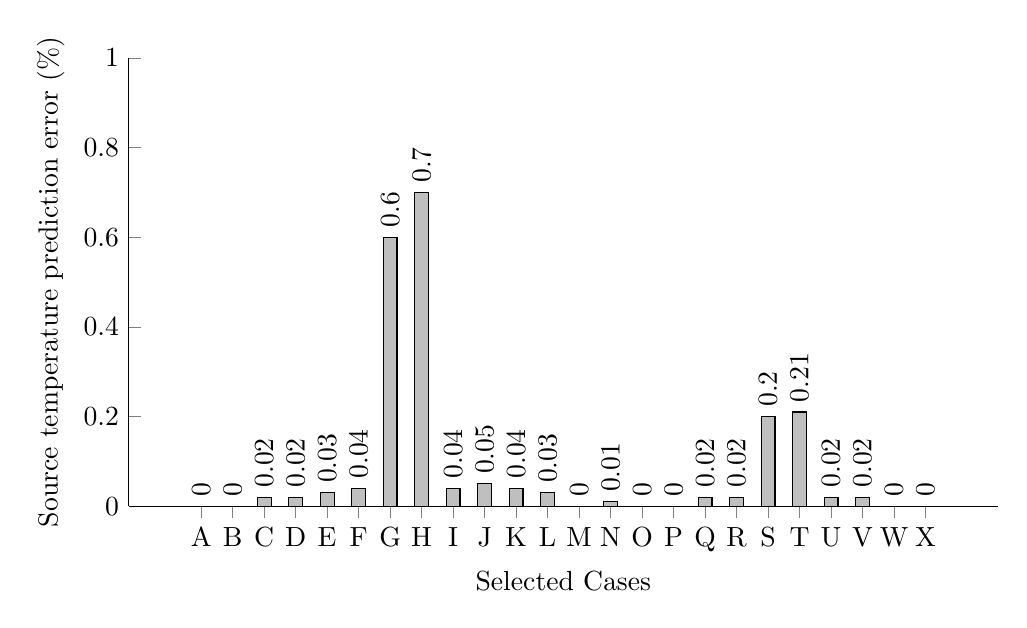
\begin{tikzpicture}
\begin{axis}[
    every axis plot post/.style={/pgf/number format/fixed},
    %ybar=5pt,
    %bar width=7pt,
    ybar=100pt,
    bar width = 5pt,
    x=0.4cm,
    ymin=0,
    axis on top,
    ymax=1,
    xtick=data,
    xlabel={Selected Cases},
	ylabel={Source temperature prediction error (\%)},
%    enlarge x limits=0.2,
    symbolic x coords={A,B,C,D,E,F,G,H,I,J,K,L,M,N,O,P,Q,R,S,T,U,V,W,X},
    restrict y to domain*=0:1.1, % Cut values off at 1.1
    visualization depends on=rawy\as\rawy, % Save the unclipped values
    nodes near coords=\rotatebox{90}{%
            \pgfmathprintnumber{\rawy}% Print unclipped values
        },
    axis lines*=left,
    clip=false
    ]
\addplot[black,fill=black!25] coordinates {
(A,0.00)(B,0.00)(C,0.02)(D,0.02)(E,0.03)(F,0.04)
(G,0.60)(H,0.70)(I,0.04)(J,0.05)(K,0.04)(L,0.03)
(M,0.00)(N,0.01)(O,0.00)(P,0.00)(Q,0.02)(R,0.02)
(S,0.20)(T,0.21)(U,0.02)(V,0.02)(W,0.00)(X,0.00)
};
\end{axis}
\end{tikzpicture}
\caption{Error in the prediction of $T_S$ from several sampled cases within the jet with $\bv{r_S}$ and $U_S$ known (min:$0\%$, max:$0.7\%$, median:$0.02\%$) \cite{vanderveer}}
\label{fig:typejetAT}
\end{center}
\end{figure}
\begin{subequations}
\begin{align}
error_{temp} (\%) &= \frac{\left|T_{SP}-T_S\right| }{T_S-T_{\infty}} \times 100 \\
error_{x-location} (\%) &= \frac{\left|x_{SP}-x_S\right|}{x_S} \times 100 \\
error_{y-location} (\%) &= \frac{\left|y_{SP}-y_S\right|}{y_S} \times 100 
\end{align}
\label{eq:error}
\end{subequations}

\subsection{Source Location and Temperature Known}
The second case is of unknown jet velocity and is also simple and breaks down to \cref{eq:Us}.  As the quadratic equation does not perfectly model the velocity profile, the error is still low, as shown in \cref{fig:typejetBU}.  The error is less than $\approx1\%$, which is generally less than that of any experimental error.
%Another simple case is that of the when the source velocity is not known.  This step also breaks down to a relatively simple equation, but this time the equation is that of \cref{eq:Us} and thus  quadratic.  This particular equation does not perfectly model the velocity profile, but as is seen in \cref{fig:typejetBU}, it is still good.  The error associated with this is never more than $\approx1\%$, which is likely less than that of any experimental error.  In this case, it is certainly less than the experimental error.  Again, the simulation parameters are described in \cref{tab:jetcases,tab:STjet}.
\begin{figure}[!t!b!p]
\begin{center}
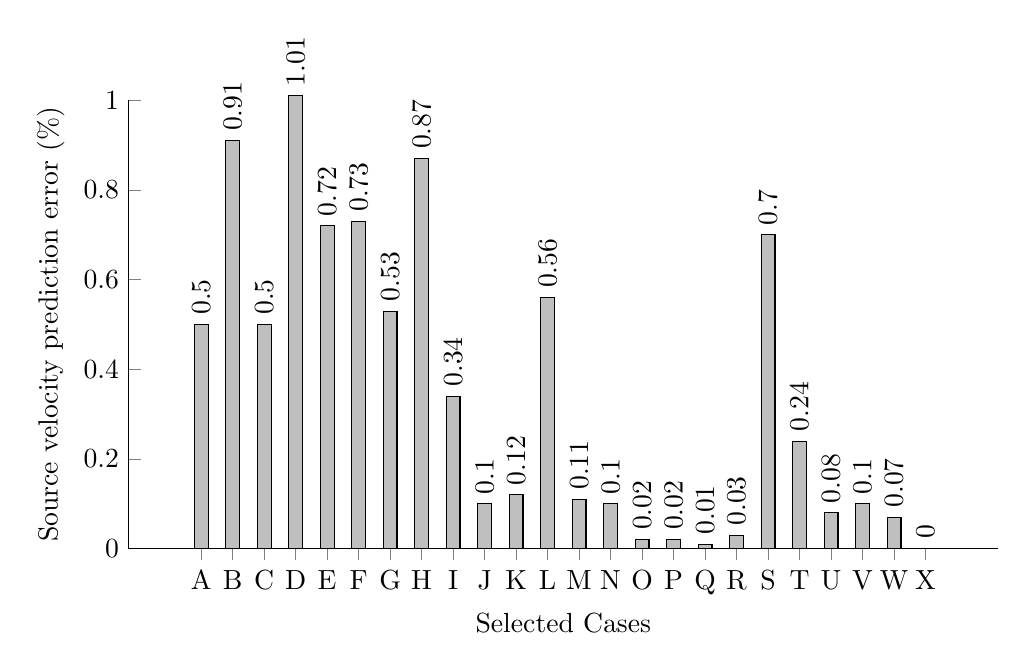
\begin{tikzpicture}
\begin{axis}[
    every axis plot post/.style={/pgf/number format/fixed},
    %ybar=5pt,
    %bar width=7pt,
    ybar=100pt,
    bar width = 5pt,
    x=0.4cm,
    ymin=0,
    axis on top,
    ymax=1,
    xtick=data,
    xlabel={Selected Cases},
	ylabel={Source velocity prediction error (\%)},
%    enlarge x limits=0.2,
    symbolic x coords={A,B,C,D,E,F,G,H,I,J,K,L,M,N,O,P,Q,R,S,T,U,V,W,X},
    restrict y to domain*=0:1.1, % Cut values off at 1.1
    visualization depends on=rawy\as\rawy, % Save the unclipped values
    nodes near coords=\rotatebox{90}{%
            \pgfmathprintnumber{\rawy}% Print unclipped values
        },
    axis lines*=left,
    clip=false
    ]
\addplot[black,fill=black!25] coordinates {
(A,0.50)(B,0.91)(C,0.50)(D,1.01)(E,0.72)(F,0.73)
(G,0.53)(H,0.87)(I,0.34)(J,0.10)(K,0.12)(L,0.56)
(M,0.11)(N,0.10)(O,0.02)(P,0.02)(Q,0.01)(R,0.03)
(S,0.70)(T,0.24)(U,0.08)(V,0.10)(W,0.07)(X,0.00)
};
\end{axis}
\end{tikzpicture}
\caption{Error in the prediction of $U_S$ from several sampled cases within the jet with $\bv{r_S}$ and $T_S$ known (min:$0\%$, max:$1.01\%$, median:$0.18\%$)\cite{vanderveer}}
\label{fig:typejetBU}
\end{center}
\end{figure}

\subsection{Source Location Known}
With only the jet location known, the method would ideally breakdown to the response surface model of \citet{knight}.  However, the methodology has the jet temperature and jet velocity solved iteratively, and must still be solved in such a manner.  The errors of the selected cases are shown in \cref{fig:typejetCT,fig:typejetCU}.  Several of the cases had a decrease in error due to the increase from one sample point to nine.


%Step three is a bit more complicated.  The method would ideally breakdown to that of the response surface model of \citet{knight}.  This however, cannot be the case as the methodology has the two equations separated and thus, they still need to be solved iteratively.  The selected cases are shown in \cref{fig:typejetCT,fig:typejetCU}, and are of the error in predicting the source temperature and velocity.  A few of the selected cases improved in accuracy due to the increase in the number of sample points.

\begin{figure}[!t!b!p]
\begin{center}
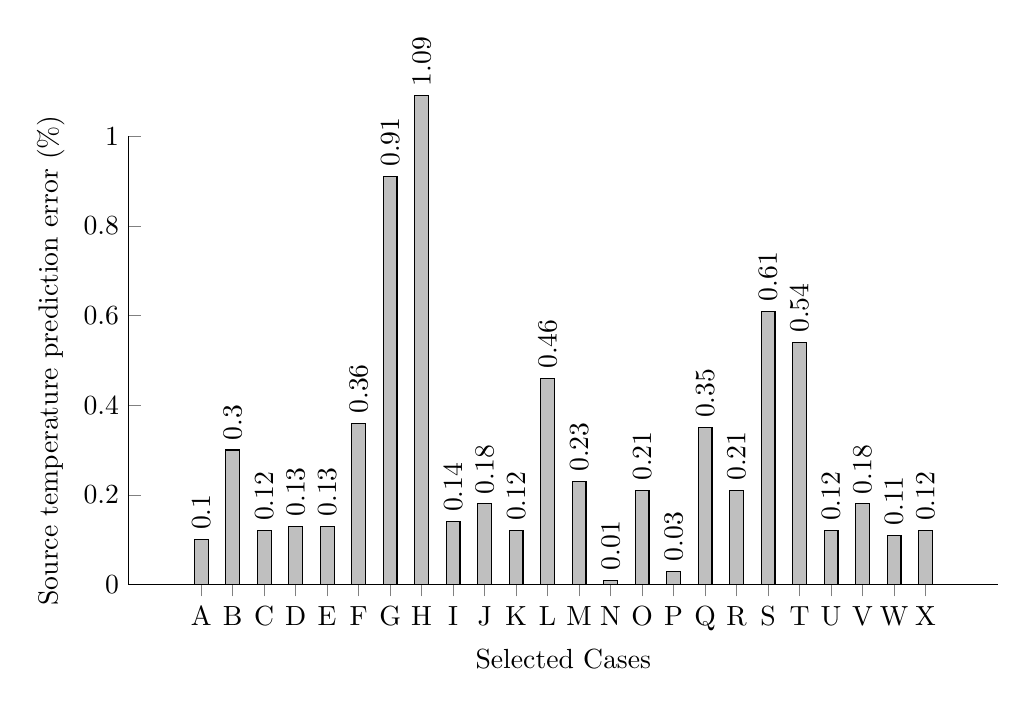
\begin{tikzpicture}
\begin{axis}[
    every axis plot post/.style={/pgf/number format/fixed},
    %ybar=5pt,
    %bar width=7pt,
    ybar=100pt,
    bar width = 5pt,
    x=0.4cm,
    ymin=0,
    axis on top,
    ymax=1,
    xtick=data,
    xlabel={Selected Cases},
	ylabel={Source temperature prediction error (\%)},
%    enlarge x limits=0.2,
    symbolic x coords={A,B,C,D,E,F,G,H,I,J,K,L,M,N,O,P,Q,R,S,T,U,V,W,X},
    restrict y to domain*=0:1.1, % Cut values off at 1.1
    visualization depends on=rawy\as\rawy, % Save the unclipped values
    nodes near coords=\rotatebox{90}{%
            \pgfmathprintnumber{\rawy}% Print unclipped values
        },
    axis lines*=left,
    clip=false
    ]
\addplot[black,fill=black!25] coordinates {
(A,0.10)(B,0.30)(C,0.12)(D,0.13)(E,0.13)(F,0.36)
(G,0.91)(H,1.09)(I,0.14)(J,0.18)(K,0.12)(L,0.46)
(M,0.23)(N,0.01)(O,0.21)(P,0.03)(Q,0.35)(R,0.21)
(S,0.61)(T,0.54)(U,0.12)(V,0.18)(W,0.11)(X,0.12)
};
\end{axis}
\end{tikzpicture}
\caption{Error in the prediction of $T_S$ from several sampled cases within the jet with $\bv{r_S}$ known (min:$0.01\%$, max:$1.30\%$, median:$0.21\%$)\cite{vanderveer}}
\label{fig:typejetCT}
\end{center}
\end{figure}

\begin{figure}[!t!b!p]
\begin{center}
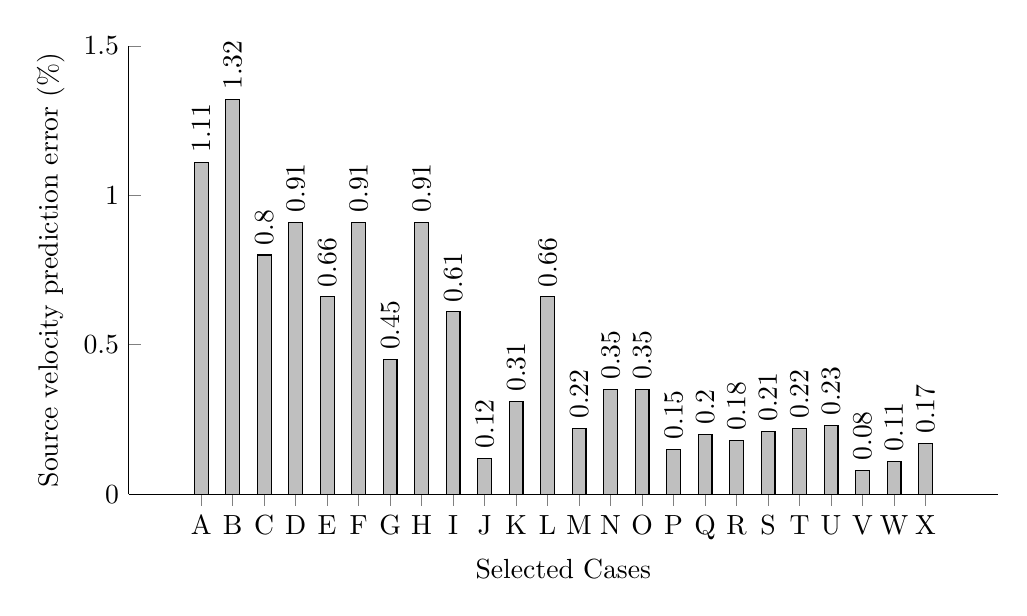
\begin{tikzpicture}
\begin{axis}[
    every axis plot post/.style={/pgf/number format/fixed},
    %ybar=5pt,
    %bar width=7pt,
    ybar=100pt,
    bar width = 5pt,
    x=0.4cm,
    ymin=0,
    axis on top,
    ymax=1.5,
    xtick=data,
    xlabel={Selected Cases},
	ylabel={Source velocity prediction error (\%)},
%    enlarge x limits=0.2,
    symbolic x coords={A,B,C,D,E,F,G,H,I,J,K,L,M,N,O,P,Q,R,S,T,U,V,W,X},
    restrict y to domain*=0:1.5, % Cut values off at 1.1
    visualization depends on=rawy\as\rawy, % Save the unclipped values
    nodes near coords=\rotatebox{90}{%
            \pgfmathprintnumber{\rawy}% Print unclipped values
        },
    axis lines*=left,
    clip=false
    ]
\addplot[black,fill=black!25] coordinates {
(A,1.11)(B,1.32)(C,0.80)(D,0.91)(E,0.66)(F,0.91)
(G,0.45)(H,0.91)(I,0.61)(J,0.12)(K,0.31)(L,0.66)
(M,0.22)(N,0.35)(O,0.35)(P,0.15)(Q,0.20)(R,0.18)
(S,0.21)(T,0.22)(U,0.23)(V,0.08)(W,0.11)(X,0.17)
};
\end{axis}
\end{tikzpicture}
\caption{Error in the prediction of $U_S$ from several sampled cases within the jet with $\bv{r_S}$ known (min:$0.08\%$, max:$1.32\%$, median:$0.33\%$)\cite{vanderveer}}
\label{fig:typejetCU}
\end{center}
\end{figure}

\subsection{Source Elevation Known}
Keeping with the incremental stepping, only the source elevation is known.  As with the previous step, nine sample points are used.  The error results of predicting the source temperature, velocity, and axial location are shown in \cref{fig:typejetDT,fig:typejetDU,fig:typejetDX}.  The max error increases significantly to $9\%$, but typical values are much less and reasonable for inverse problems.


%This is the next logical step, and only the source elevation is known a priori.  \Cref{fig:typejetDT,fig:typejetDU,fig:typejetDX} are bar charts containing the error associated with predicting the source temperature, velocity, and axial location, respectively.  The charts are of the same selected cases of \cref{tab:jetcases}.  The error is significantly increased to higher than $9\%$ for predicting the source velocity.  Even an error of $9\%$ is still reasonable, but the methodology does not seem to function as well for the jet in a crossflow problem.  This is likely due to not utilizing an optimized search shape for the jet, even though nine sample points were used.  
%
%\Cref{fig:typejetEUTX} contains a plot of the predicted vs actual jet temperature.  \Cref{fig:typejetEXTU} is a similar plot for jet velocity.
%
\begin{figure}[!t!b!p]
\begin{center}
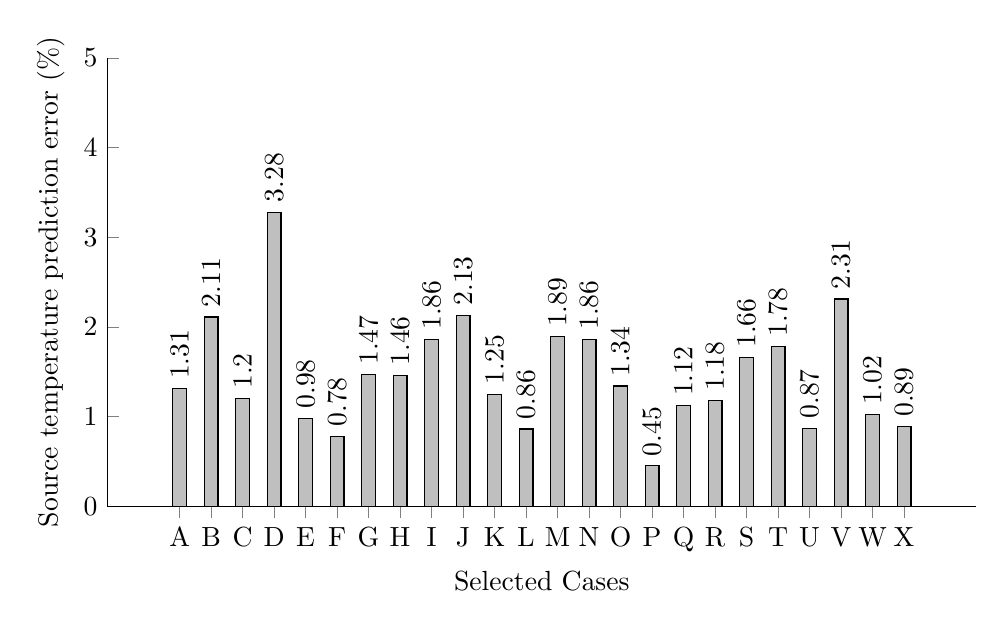
\begin{tikzpicture}
\begin{axis}[
    every axis plot post/.style={/pgf/number format/fixed},
    %ybar=5pt,
    %bar width=7pt,
    ybar=100pt,
    bar width = 5pt,
    x=0.4cm,
    ymin=0,
    axis on top,
    ymax=5,
    xtick=data,
    xlabel={Selected Cases},
	ylabel={Source temperature prediction error (\%)},
%    enlarge x limits=0.2,
    symbolic x coords={A,B,C,D,E,F,G,H,I,J,K,L,M,N,O,P,Q,R,S,T,U,V,W,X},
    restrict y to domain*=0:5.1, % Cut values off at 1.1
    visualization depends on=rawy\as\rawy, % Save the unclipped values
    nodes near coords=\rotatebox{90}{%
            \pgfmathprintnumber{\rawy}% Print unclipped values
        },
    axis lines*=left,
    clip=false
    ]
\addplot[black,fill=black!25] coordinates {
(A,1.31)(B,2.11)(C,1.20)(D,3.28)(E,0.98)(F,0.78)
(G,1.47)(H,1.46)(I,1.86)(J,2.13)(K,1.25)(L,0.86)
(M,1.89)(N,1.86)(O,1.34)(P,0.45)(Q,1.12)(R,1.18)
(S,1.66)(T,1.78)(U,0.87)(V,2.31)(W,1.02)(X,0.89)
};
\end{axis}
\end{tikzpicture}
\caption{Error in the prediction of $T_S$ from several sampled cases within the jet with source elevation known (min:$0.45\%$, max:$3.28\%$, median:$1.32\%$)\cite{vanderveer}}
\label{fig:typejetDT}
\end{center}
\end{figure}
%
\begin{figure}[!t!b!p]
\begin{center}
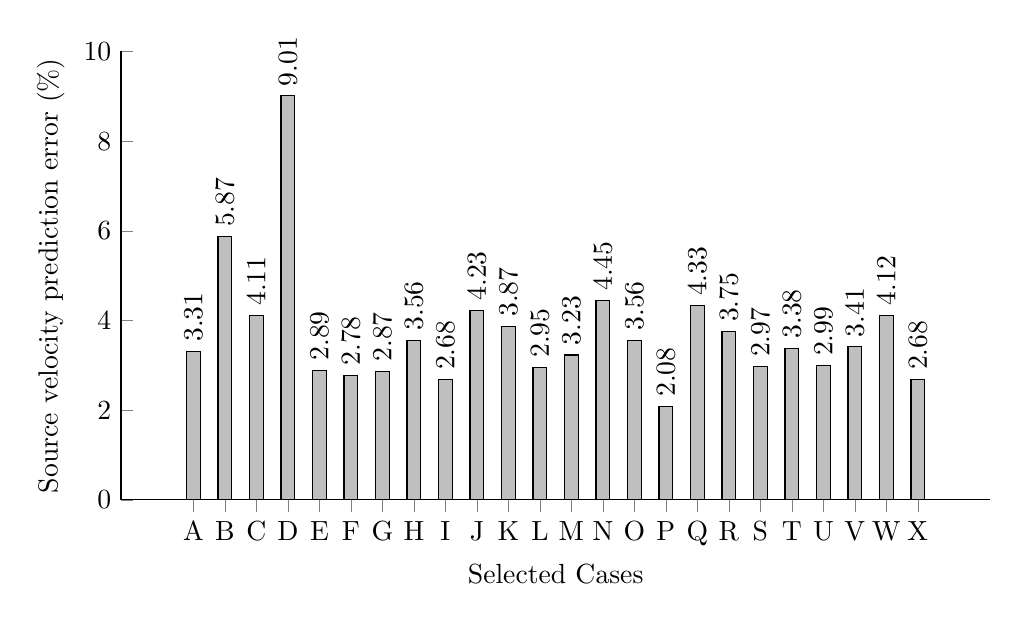
\begin{tikzpicture}
\begin{axis}[
    every axis plot post/.style={/pgf/number format/fixed},
    %ybar=5pt,
    %bar width=7pt,
    ybar=100pt,
    bar width = 5pt,
    x=0.4cm,
    ymin=0,
    axis on top,
    ymax=10,
    xtick=data,
    xlabel={Selected Cases},
	ylabel={Source velocity prediction error (\%)},
%    enlarge x limits=5.2,
    symbolic x coords={A,B,C,D,E,F,G,H,I,J,K,L,M,N,O,P,Q,R,S,T,U,V,W,X},
    restrict y to domain*=0:10.1, % Cut values off at 1.1
    visualization depends on=rawy\as\rawy, % Save the unclipped values
    nodes near coords=\rotatebox{90}{%
            \pgfmathprintnumber{\rawy}% Print unclipped values
        },
    axis lines*=left,
    clip=false
    ]
\addplot[black,fill=black!25] coordinates {
(A,3.31)(B,5.87)(C,4.11)(D,9.01)(E,2.89)(F,2.78)
(G,2.87)(H,3.56)(I,2.68)(J,4.23)(K,3.87)(L,2.95)
(M,3.23)(N,4.45)(O,3.56)(P,2.08)(Q,4.33)(R,3.75)
(S,2.97)(T,3.38)(U,2.99)(V,3.41)(W,4.12)(X,2.68)
};
\end{axis}
\end{tikzpicture}
\caption{Error in the prediction of $U_S$ from several sampled cases within the jet with source elevation known (min:$2.08\%$, max:$9.01\%$, median:$3.40\%$)\cite{vanderveer}}
\label{fig:typejetDU}
\end{center}
\end{figure}
%
\begin{figure}[!t!b!p]
\begin{center}
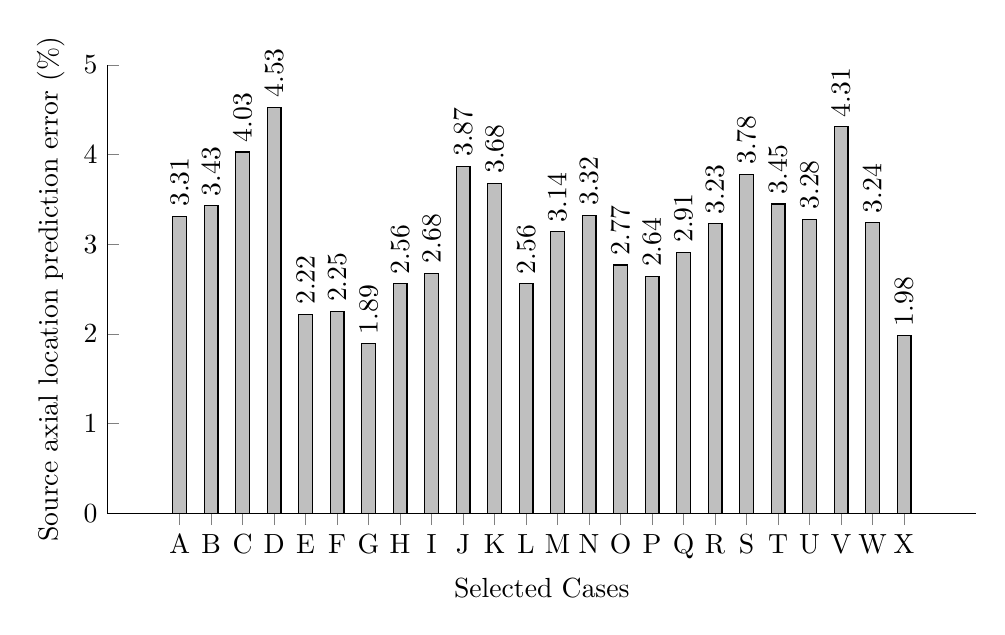
\begin{tikzpicture}
\begin{axis}[
    every axis plot post/.style={/pgf/number format/fixed},
    %ybar=5pt,
    %bar width=7pt,
    ybar=100pt,
    bar width = 5pt,
    x=0.4cm,
    ymin=0,
    axis on top,
    ymax=5,
    xtick=data,
    xlabel={Selected Cases},
	ylabel={Source axial location prediction error (\%)},
%    enlarge x limits=0.2,
    symbolic x coords={A,B,C,D,E,F,G,H,I,J,K,L,M,N,O,P,Q,R,S,T,U,V,W,X},
    restrict y to domain*=0:5.1, % Cut values off at 1.1
    visualization depends on=rawy\as\rawy, % Save the unclipped values
    nodes near coords=\rotatebox{90}{%
            \pgfmathprintnumber{\rawy}% Print unclipped values
        },
    axis lines*=left,
    clip=false
    ]
\addplot[black,fill=black!25] coordinates {
(A,3.31)(B,3.43)(C,4.03)(D,4.53)(E,2.22)(F,2.25)
(G,1.89)(H,2.56)(I,2.68)(J,3.87)(K,3.68)(L,2.56)
(M,3.14)(N,3.32)(O,2.77)(P,2.64)(Q,2.91)(R,3.23)
(S,3.78)(T,3.45)(U,3.28)(V,4.31)(W,3.24)(X,1.98)
};
\end{axis}
\end{tikzpicture}
\caption{Error in the prediction of $x_S$ from several sampled cases within the jet with source elevation known (min:$1.89\%$, max:$4.53\%$, median:$3.24\%$)\cite{vanderveer}}
\label{fig:typejetDX}
\end{center}
\end{figure}


\subsection{Source Location and Strength Unknown}
The final incremental step is not possible with the current methodology and search shape.  The underlying, self-similar characteristics of a jet in a crossflow creates an indiscernible infinite set of possible solutions.  It is possible that a significant increased sample size would alleviate the problem, but the goal of this work was to utilize very limited domain information.

As an example, a set of alternate solutions is shown in \cref{tab:alternatives} for case `V'.  This list was not meant to be comprehensive, but rather illustrative of the problem.  The last column is the percent error between the various solutions.

%The last step with source location and strength unknown is not possible with the current search shape and methodology.  The issue in this case is the self-similar nature of a jet in a crossflow, where there are multiple solutions to the problem.  That is to say that the nine point search shape can converge on multiple solutions.  

%This is similar to the problem with the plume in a crossflow prior to using the new optimized search shape.  In that problem, the solutions all had the same predicted source temperature, with different locations with the same search shape.  This problem has completely unique solutions with the same search shape.

%When searching the domain for alternative solutions, a search space of $350-450\,K$ in $25\,K$ increments and $0-4\,m/s$ in $0.5\,m/s$ increments were used.  Take the `V' case for example, there are nine alternative solutions with less than $1\%$ error difference between the search shape temperatures.  \Cref{tab:alternatives} is a list of all of the alternatives, including the `V' case at the top of the table.  The alternatives seem to be discernible knowing the elevation, which is why the previous step was able to be resolved.

\begin{table}[!t!b!p]
\begin{center}
\begin{tabular}{ l l l l l }
\hline
Axial    		& Elev.		& Jet		  	& Jet			& Search Shape \\
Loc. $(mm)$ & Loc. $(mm)$	& Temp. $(K)$ 	& Vel. $(m/s)$	& Error $(\%)$\\ \hline
20.0 &	3.0	&	425	&	2.0	&	0.00 \\ \hline
10.0 &  3.7 &	375 &	2.5 &	0.60 \\
12.0 &	5.1 &	375	&	3.0	&	0.34 \\
14.8 &	2.7 &	400	&	2.0	&	0.30 \\
16.3 &	4.5 &	400	&	2.5	&	0.26 \\
19.5 &	5.9 &	400	&	3.0	&	0.29 \\
21.8 &	5.0 &	425	&	2.5	&	0.24 \\
25.6 &	6.5 &	425	&	3.0	&	0.34 \\
25.2 &	3.2 &	450	&	2.0	&	0.13 \\
26.8 &	5.4 &	450	&	2.5	&	0.25 \\
\hline
\end{tabular}
\caption{Example alternative solutions\cite{vanderveer}}
\label{tab:alternatives}
\end{center}
\end{table}

\subsection{Experimental Results}
Due to the last step we will only consider searching for the source temperature, velocity, and axial location for the experimental cases.  The experimental conditions are listed in \cref{tab:ETjet}.  A select few results are shown in \cref{tab:typejetF}.  A table format was chosen to represent the data, as the error is significant and would make a chart difficult to read.  The axial direction error has a minimum of $5.4\%$, a maximum of $18.7\%$, and a median of $10.5\%$.  The jet velocity error has a minimum of $10.4\%$, a maximum of $21.8\%$, and a median of $14.75\%$.  The jet temperature error has a minimum of $8.64\%$, a maximum of $13.7\%$, and a median of $9.99\%$.

A graph of actual vs predicted source temperature and velocity are shown in \cref{fig:typejetEUTXEE,fig:typejetEXTUEE} respectively.  It is easily visualized that this methodology predicts the source velocity significantly better than source temperature.  The large percentages are due to the velocities being small.  Often, the predicted error is close to the experimental error of the system.

%Due to the issue in determining the four unknowns, the experimental results are limited to finding only axial location and source strength.  The conditions of the experiments are shown in \cref{tab:ETjet}.  The results from a few select cases are shown in \cref{tab:typejetF}.  Due to the severe addition of error to the experimental results, the results are shown in a table format rather than the previously used bar graphs.

%The error predicting the axial location is as high as $18.7\%$.  The error in predicting source velocity is as high as $21.8\%$.  The error for source temperature is as high as $13.7\%$.  These high error rates should be expected, as there are many contributing factors.  The search shape is not optimized for the jet, the number of sample points may not be enough, and the simulations do not exactly follow the experiment.  Even with these issues, the methodology was able to predict close to, if not within, experimental error.  Realize that $20\%$ of $1.0\,m/s$ is the accuracy of the experimental jet velocity.
%
%The comparison of actual vs predicted jet temperature and velocity is shown in \cref{fig:typejetEUTXEE} and \cref{fig:typejetEXTUEE}
%
\begin{table}[!t!b!p]
\begin{center}
\begin{tabular}{ c c }
\hline
Parameter    & Value \\ \hline
$T_{\infty} \, (K) $ & $297.6\pm8.0$ \\
$P_{\infty} \, (kPa) $ & $100.6\pm0.6$ \\ 
$U_{\infty} \, (m/s) $ & $2.0\pm0.02$ \\ \hline
\end{tabular}
\caption{Experimental test conditions}
\label{tab:ETjet}
\end{center}
\end{table}
%
\begin{table}[!h!t!b!p]
\begin{center}
\begin{tabular}{ l | l c c c c}
\hline
 $U_{S}$ $(m/s)$ & & 1.0 & 1.0 & 4.0 & 4.0 \\ \hline
 $T_S$ $(K)$ & & 375 & 425 & 375 & 425  \\ \hline \hline
 Location (x,y) & \\
 10 mm, 0 mm & X & $10.9\%$ & $11.7\%$ & $11.1\%$ & $13.8\%$ \\
 			 & U & $21.8\%$ & $18.6\%$ & $10.4\%$ & $11.9\%$ \\
 			 & T & $8.70\%$ & $9.87\%$ & $10.7\%$ & $12.9\%$ \\ \hline
 20 mm, 0 mm & X & $8.65\%$ & $7.65\%$ & $5.40\%$ & $9.81\%$ \\
 			 & U & $18.7\%$ & $19.8\%$ & $11.5\%$ & $12.1\%$ \\
 			 & T & $8.81\%$ & $10.7\%$ & $9.65\%$ & $10.2\%$ \\ \hline
 30 mm, 0 mm & X & $10.6\%$ & $10.4\%$ & $18.7\%$ & $9.78\%$ \\
 			 & U & $15.8\%$ & $17.9\%$ & $12.3\%$ & $13.7\%$ \\
 			 & T & $9.61\%$ & $8.64\%$ & $13.7\%$ & $10.1\%$ \\ \hline			 
 \end{tabular}
\caption{Error in predicting source axial location ($x_S$), source strength($U_S$ and $T_S$) from a few sample cases within the jet, search shape with 9pts, utilizing experimental data\cite{vanderveer}}
\label{tab:typejetF}
\end{center}
\end{table}

\begin{figure}[!h!t!b!p]
\begin{center}
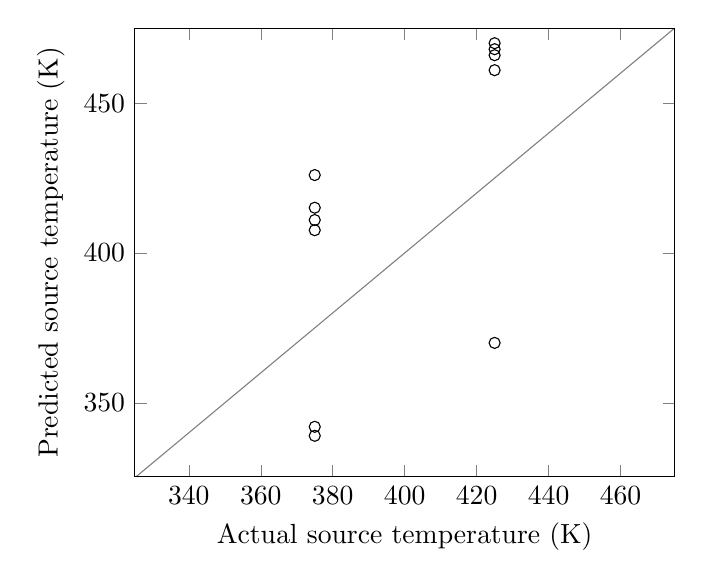
\begin{tikzpicture}
\begin{axis}[
    every axis plot post/.style={/pgf/number format/fixed},
%    ymin=325,
    axis on top,
    ymax=475,
    xmax=475,
    xmin=325,
    xlabel={Actual source temperature (K)},
	ylabel={Predicted source temperature (K)}]
	\addplot[only marks,draw=black,mark=o] coordinates {
		(375,407.6)(375,415.1)(375,342)(375,411)(375,339)(375,426)(425,466)(425,370)(425,470)(425,468)(425,461) %(425,467)
		};
	\addplot[draw=gray] coordinates {
		(300,300) (500,500)		
		};	
\end{axis}
\end{tikzpicture}
\caption{Actual vs predicted source temperature for several cases within the jet}
\label{fig:typejetEUTXEE}
\end{center}
\end{figure}
\begin{figure}[!h!t!b!p]
\begin{center}
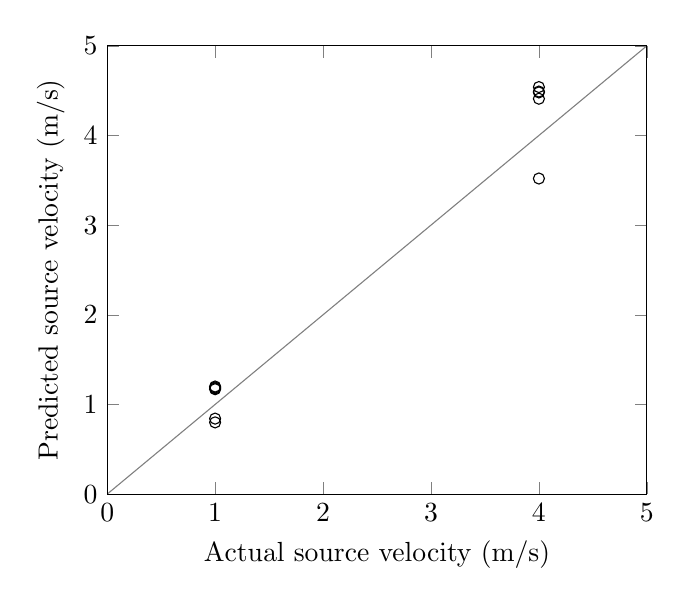
\begin{tikzpicture}
\begin{axis}[
    every axis plot post/.style={/pgf/number format/fixed},
    ymin=0,
    axis on top,
    ymax=5,
    xmax=5,
    xmin=0,
    xlabel={Actual source velocity (m/s)},
	ylabel={Predicted source velocity (m/s)}]
	\addplot[only marks,draw=black,mark=o] coordinates {
		(1,1.2)(1,1.18)(1,0.8)(1,1.19)(1,.842)(1,1.17)(4,4.41)(4,3.52)(4,46)(4,4.48)(4,4.49)(4,4.54)
		};
	\addplot[draw=gray] coordinates {
		(0,0) (5,5)		
		};	
\end{axis}
\end{tikzpicture}
\caption{Actual vs predicted source velocity for several cases within the jet}
\label{fig:typejetEXTUEE}
\end{center}
\end{figure}
\section{Conclusions}
A predictor-corrector method was modified and applied to the inverse jet in a crossflow problem.  The inverse method was previously developed and the search shape was optimized.  Four parameters were searched for source temperature, velocity, axial location, and elevation.  The new methodology functioned accurately for 4 out of 5 steps, with all four parameters unknown being the exception.  There was not enough information to accurately discern the solution from the infinite solution set.  Other than the exception, the methodology performed well with approximately $9\%$ even in the worst cases, and typically performing much better.

The step utilizing experimental results showed a greater error.  This indicates that this methodology, when applied to the jet in a crossflow problem, is error sensitive.  The error was as large as $21.8\%$ for the jet velocity and as small as $5.4\%$ for the axial location of the jet.

Previous optimization of the search shape indicates that the methodology is sensitive to the search shape\cite{ijhmt2}.  More work on the inverse jet in a crossflow problem, by optimizing the search shape specifically for the jet problem, may reduce the overall error.

The methodology has demonstrated its capabilities and limitations, and much more work may be done regarding the limitations.  There are several improvements still needing to be made, such as three dimensional capabilities, transient capabilities, and possibly the ability to differentiate multiple sources.  These features, if implemented, would have significant applications to fires in urban environments and pollution in industrial areas.
\appendix

\bibliography{Bibliography}{}
\bibliographystyle{model1-num-names}
\end{document}

